\documentclass{beamer}
\usetheme{Boadilla}
\title[Semester Project]{Rigorous data-driven computation of spectral properties of Koopman operators for dynamical systems}
\subtitle{Based on an article by Matthew J. Colbrook and Alex Townsend \cite{colbrook_rigorous_2021}}
\author[Ivan Bioli]{\emph{Author} : Ivan Bioli\\[5mm]{\emph{Professor} : Daniel Kressner \\ \emph{Supervisor} : Alice Cortinovis}}
\institute[EPFL]{École Polytechnique Fédérale de Lausanne\\Master in Computational Sciences and Engineering}
\date{May 30, 2022}
\usepackage{preamble_presentation}
\setbeamertemplate{caption}{\insertcaption}

\usepackage{pgfpages}
\setbeameroption{show notes on second screen}

\begin{document}
\begin{frame}
\centering
\titlepage
\end{frame}

\begin{frame}[fragile]{The Koopman Operator}
Autonomous dynamical systems with finite-dimensional state space and discrete time steps:
\begin{equation*}
    \vb{x}_{n+1} = \vb{F}(\vb{x}_n)\,\,\,n\geq 0, \qquad \vb{F}:\Omega \to \Omega
\end{equation*}
\begin{definition}[Observable]
A function $g:\Omega\to\C$ used to indirectly measure the state of the dynamical system is called an observable. 
\end{definition}
\begin{definition}[Koopman Operator]
Given a suitable domain of observables $\mathcal{D}(\mathcal{K}) \subseteq L^2(\Omega)$ we define the Koopman Operator as:
\begin{equation*}
    \label{koopman_def}
    \begin{split}
       \mathcal{K} : \mathcal{D}(\mathcal{K}) &\longrightarrow L^2(\Omega, \omega)
       \\
       g & \longmapsto g \circ \vb{F}
    \end{split}    
\end{equation*} 
\end{definition}
\end{frame}

\note[itemize]{
\item Throughout this work, we will consider autonomous dynamical systems with finite-dimensional state space $\Omega\subseteq \R^d$ and discrete time steps according to a function F.
\item In a data-drive perspective, we deal with measurements of the system states. These measurements are nothing more than functions of the system states, hence the concept of observable. 
\item We can think of the Koopman Operator as lifting the dynamics from the state space to the space of observables. 
\item From this lifting, we gain that, regardless of the linearity or nonlinearity of F, the Koopman Operator is a linear operator and therefore, to understand the dynamics of the system, we can analyze the spectral properties of $\mathcal{K}$. 
\item However, the disadvantage is that the space of the observables is infinite-dimensional.
}

\begin{frame}[fragile]{Linear dynamical systems}
\centering
$\vb{F}(\vb{x}) = A\vb{x}$, $\vb{A}\in\R^{d\times d}$
\begin{prop}
Let us assume that $\vb{A}\in\R^{d\times d}$ is diagonalizable with a full set of eigenpairs $\{(\lambda_j, \vb{v}_j)\}_{j=1}^{d}$. Let $\{(\overline{\lambda}_j, \vb{w}_j)\}_{j=1}^{d}$ be the eigenpairs of of $\vb{A}^*$, with $\{\vb{w}_j)\}_{j=1}^{d}$ such that $\langle \vb{v}_j, \vb{w}_k\rangle = \delta_{k,j}$. Then we can rewrite $\vb{x}\in\R^d$:
\begin{equation*}
    \label{decomposition_linear}
    \vb{x} = \sum_{j=1}^d \langle \vb{x}, \vb{w}_j\rangle \vb{v}_j = \sum_{j=1}^d \phi_j(\vb{x}) \vb{v}_j.
\end{equation*}
It holds $[\mathcal{K}\phi_j](\vb{x}) = \lambda_j\phi_j$ and the evolution of the system reads
\begin{equation*}
    \label{evolution_linear}
    \vb{F}(\vb{x}) = \vb{A}\vb{x}  = \sum_{j=1}^d \phi_j(\vb{x}) \vb{A}\vb{v}_j = \sum_{j=1}^d \lambda_j \phi_j(\vb{x}) \vb{v}_j = \sum_{j=1}^d [\mathcal{K}\phi_j](\vb{x})\vb{v}_j.
\end{equation*}
\end{prop}
\end{frame}

\note[itemize]{
\item Let us first consider the case of linear dynamical systems. If the matrix A is diagonalizable, as summarized in this proposition, we can recover the eigenpairs of the Koopman operator from the left eigenvectors of A.
\item Moreover, we can write each vector as here. The decomposition is nothing more than an expansion of x as a linear combination of the vectors $v_j$ , where the $\phi_j(x)$ are the coefficients. However, from the Koopman Operator’s viewpoint, it is a linear expansion of the (vector) full state observable as a linear combination of the eigenfunctions of $\mathcal{K}$, where now the role of the coefficients is played by the vectors $v_j$.
\item This gives the idea to define the Koopman mode decomposition
}

\begin{frame}[fragile]{Nonlinear dynamical systems}
\begin{definition}[Koopman Mode Decomposition]
$g:\Omega\to\C^p$ a vector valued observable s.t. each of its component $g_i$ lies in the closure of the Span of $J$ Koopman eigenfunctions, where the case $J=+\infty$ is possible (and often occurs). Then we can write $\displaystyle{g_i = \sum_{j = 1}^J v_{ij}\phi_j, \, v_{ij}\in\C}$ and staking the weights into the vectors 
%$\vb{v}_j = [v_{1j},\dots,v_{pj}]^T\in\C^p$ 
\begin{equation*}
    \label{koopman_modes}
	g(\vb{x}) = \sum_{j = 1}^J \phi_j(\vb{x})\vb{v}_{j}.
\end{equation*}
\end{definition}
\begin{itemize}
    %\item $\vb{F}(\vb{x}) = [\mathcal{K}g](\vb{x}) = \sum_{j = 1}^J [\mathcal{K}\phi_j](\vb{x})\vb{v}_j = \sum_{j = 1}^J \lambda_j\phi_j(\vb{x})\vb{v}_j$
    \item $g(\vb{x}_n) = [\mathcal{K}^ng](\vb{x}_0) = \sum_{j = 1}^J \lambda_j^n\phi_j(\vb{x}_0)\vb{v}_{j}$ 
    %\item Idea: link the two formulations via the full state observable $g(x) = x$
\end{itemize}
\end{frame}
\note[itemize]{
\item We can think of a vector valued observable g as a vector gathering different measurements of the system state. Thehen we can write ... and the vectors $v_j$, which play the role of the coefficients as before, are called Koopman modes.
\item By linearity of the Koopman operator, the evolution of the observable is ...
\item From here we can understand that the Koopman eigenvalue $\lambda_j$ characterizes the contribution of the corresponding Koopman mode $v_j$ to the evolution of the observable over time: the phase of $\lambda_j$ determines its frequency, while the magnitude determines the growth rate.
}

\begin{frame}[fragile]{Dynamic Mode Decomposition (DMD)}
Linear dynamical system: $x_{n+1} = Ax_n$. Access to a sequence of snapshots:
\begin{equation*}
    \vb{V}_1^N = \left[\vb{v}_1, \vb{v}_2, \dots, \vb{v}_N\right] = \left[\vb{v}_1, \vb{A}\vb{v}_1, \dots, \vb{A}^N\vb{v}_1\right]
\end{equation*}
\alert{\textbf{Idea:}} write $\vb{v}_N = a_1 \vb{v}_1 + \dots + a_{N-1} \vb{v}_{N-1} + \vb{r}$ and minimize the residual.
\begin{block}{DMD (Arnoldi-based version)}
\begin{equation*}
    \vb{A}\vb{V}_1^{N-1}  = \vb{V}_1^{N-1}\vb{S} + \vb{r}\vb{e}_{N-1}^T, \quad 
    \vb{S} :=
   \begin{bmatrix}
   0     &        &       &      & a_1 \\
   1     & 0      &       &      & a_2 \\
         & \ddots & \ddots&      & \vdots \\ 
         &        & 1     & 0    & a_{N-2} \\
         &        &       & 1    & a_{N-1} \\
   \end{bmatrix}.
\end{equation*}
To minimize the norm of the residual $\vb{V}_1^{N-1} = \vb{Q}\vb{R}$ and:
\begin{equation*}
    \vb{a} = \vb{R}^{-1} \vb{Q}^*\vb{v}_N = (\vb{V}_1^{N-1})^{\dagger}\vb{v}_N.
\end{equation*}
\end{block}
\end{frame}

\note[itemize]{
\item As already discussed, in order to extract the dynamic characteristics we need to analyze the spectral properties of A. However, in a data-drive perspective, we cannot assume that we have access to A, but only to a sequence of snapshots. As we do not have access to the matrix A and we cannot compute products of vectors by this matrix, we cannot directly apply numerically stable algorithms such as the Arnoldi method, and we can rely only on the sequence of snapshots we are given in input.
\item In general, $v_N$ does not necessarily belong to the Span of the columns of $\vb{V}_1^{N-1}$
1. However, as N increases the snapshots tend to lie in the same direction (or at least in the same subspace).
\item We can write this in term of a companion matrix S and then minimize the residual solving the corresponding least squares problem. The eigenpairs of A are then approximated by those of S.

}

\begin{frame}{DMD and the Arnoldi method}
\begin{prop}
Suppose that $\vb{V}_1^{N-1}$ is of full column rank. Then the Arnoldi method and the DMD algorithms are equivalent in exact arithmetic, i.e. the Ritz pairs returned by the two algorithms coincide. 
\end{prop}
\alert{\textbf{But:}} the Arnoldi method is more stable as does not compute the iterates explicitly. A SVD-based version of the DMD algorithm improves numerical stability (and is equivalent in exact arithmetic).
\begin{figure}[h]
    \begin{columns}
        \column{.45\linewidth}
        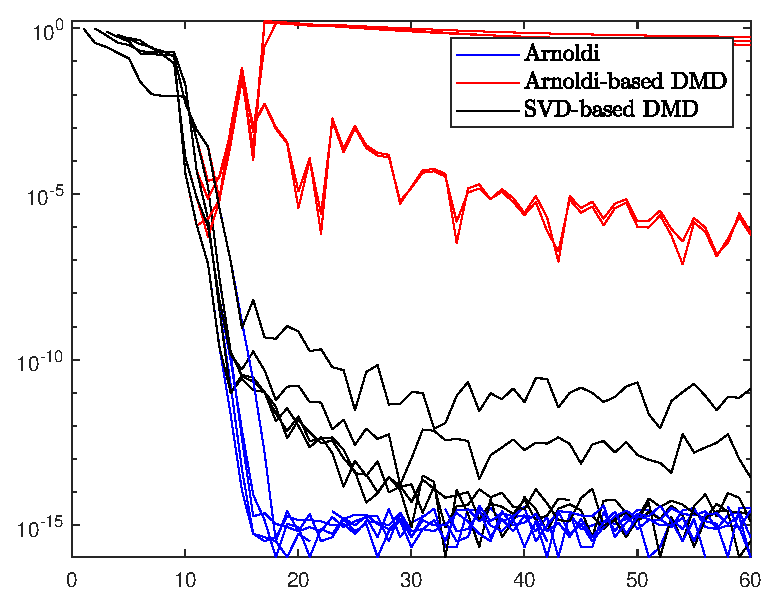
\includegraphics[width=\linewidth]{../code/figures/Arnoldi_vs_DMD.eps}
        \column{.5\linewidth}
        \caption{Convergence of the five dominant eigenvalues using a matrix \texttt{A} of size \texttt{n = 400} defined as:\\ \texttt{A = diag([1, 0.9, 0.8.\^{}(1:n-2)])}.}
      \end{columns}
\end{figure}
\end{frame}

\note[itemize]{
\item Although the two algorithms are equivalent mathematically and in exact arithmetic, the Arnoldi algorithm is numerically more stable. Indeed, as the number of snapshots increases, the vectors tend to become linearly dependent and therefore, the matrix $\vb{V}_1^{N}$ becomes close to singular, hence ill conditioned.
\item One of the major strengths of the Arnoldi algorithm is that it does not even compute the vectors $v_j$ because errors are already made in these computations. However, in a data-driven perspective, this is not possible since what we are given is a sequence of snapshots and not the matrix A. Hence, we trade-off better stability and convergence properties for an algorithm that only relies on $\vb{V}_1^{N-1}$ and is therefore applicable to snapshots experimentally collected
\item Using an equivalent SVD-based version of DMD improves numerical stability as it can be seen from this figure
}

\begin{frame}{Extended Dynamic Mode Decomposition (EDMD)}
\alert{\textbf{Idea:}} approximate the Koopman Operator as a finite dimensional operator and then approximate the Koopman (eigenvalue, eigenfunction, mode) tuples from this finite dimensional approximation. 

\medskip
\structure{\textbf{Input}}:
\begin{itemize}
    \item Snapshot pairs of the system state: $\{(\vb{x}_0^{(m)}, \vb{x}_1^{(m)})\}_{m = 1}^M$ with $\vb{x}_1^{(m)} = \vb{F}(\vb{x}_0^{(m)})$;
    \item a dictionary of observables $\mathcal{D} = \{\psi_1, \dots, \psi_K\} \subseteq \mathcal{D}(\mathcal{K})$.
\end{itemize}
\begin{columns}[T] % align columns
\begin{column}{.48\textwidth}
{\usebeamercolor[fg]{structure}\textbf{DMD}\\\vspace{-6pt}\rule{\linewidth}{2pt}}
{\footnotesize
\begin{equation*}
    \begin{split}
        \Psi_0 &= \left[\Psi(\vb{x}_0^{(1)}), \dots, \Psi(\vb{x}_0^{(M)})\right]\\
        \Psi_1 &= \left[\Psi(\vb{x}_1^{(1)}), \dots, \Psi(\vb{x}_1^{(M)})\right] = \\
        & = \left[[\mathcal{K}\Psi](\vb{x}_0^{(1)}), \dots, [\mathcal{K}\Psi](\vb{x}_0^{(M)})\right] \\
        K &= \Psi_1\Psi_0^{\dagger}
    \end{split}
\end{equation*}}
\end{column}%
\hfill%
\begin{column}{.48\textwidth}
{\usebeamercolor[fg]{structure}\textbf{EDMD}\\\vspace{-6pt}\rule{\linewidth}{2pt}}
{\footnotesize
\begin{equation*}
    \begin{split}
        &\phi = \sum_{k=1}^K a_k\psi_k = \Psi^T\vb{a}, \quad \vb{a}\in\C^K \\
        &\mathcal{K}\vb{\phi} = (\Psi^T \circ \vb{F})\vb{a} = \Psi^T\vb*K\vb{a} + r\\
        &\min_{\vb*{K}\in\C^{K\times K}}\int_{\Omega} \max_{\vb{a}\in\C^k,\,\norm{\vb{a}} = 1}\abs{r(\vb{a}, \vb{x})}^2 d\omega(\vb{x})
    \end{split}
\end{equation*}}
\end{column}%
\end{columns}
\end{frame}

\note[itemize]{
{\footnotesize
\item Until now we focused on the linear setting. However, it is in the nonlinear one that the Koopman operator provides the greatest advantages by linearizing the dynamics.
\item In analogy to what has been done in the linear case, we compute the observable $\Psi$ on the datapoints and $K = \Psi_1\Psi_0^{\dagger}$ provides the best finite-dimensional approximation of the Koopman operator that can be achieved using the available data. Therefore, we can approximate the Koopman eigenvalues and modes from the eigendecomposition of K.
\item The interpretation of K as the best finite-dimensional approximation of the Koopman Operator gives an idea of why Algorithm 2 might work. However, this does not provide a mathematical foundation for the method and for why it should perform well in a strongly nonlinear dynamics. 
\item The key idea of EDMD is to directly move in the functional setting. We consider $\phi\in\Span(D)$, we approximate the dynamics on $\Span(D)$ by a matrix K, and we minimize the norm of the point-wise maximum of the residual of all possible $\phi\in\Span(D)$. If one approximates the integral using the snapshots as quadrature points, a least squares problem arises and this leads to the so called EDMD.}
}

\begin{frame}{A 1D example: the Gauss iterated map}
\begin{equation*}
    F:\Omega = [-1, 0] \to\Omega, \qquad F(x) =\exp(\alpha x^2) + \beta 
\end{equation*}
We consider:
\begin{itemize}
    \item $\{\vb{x}_0^{(m)}\}_{m = 1}^M$: Gauss-Legendre quadrature nodes, $M = 100$.
    \item Dictionary of observable $\mathcal{D}$: first $K = 40$ normalized Legendre polynomials, transplanted to $\Omega$.
\end{itemize}
\begin{figure}[h]
    \centering
    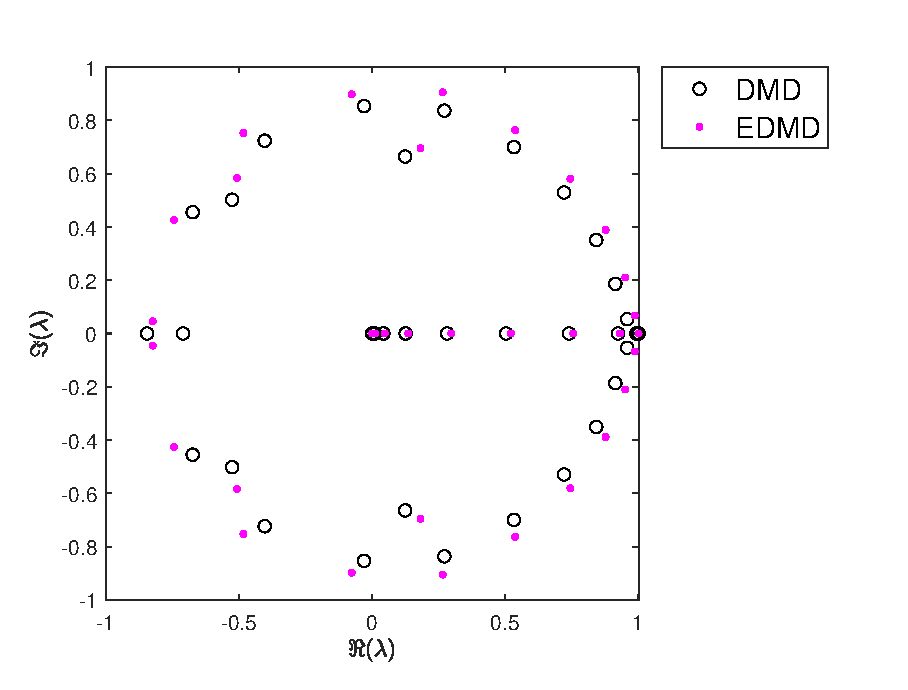
\includegraphics[width=0.55\linewidth]{../code/figures/gauss_map/presentation.eps}
\end{figure}
\end{frame}

\note[itemize]{
\item Let us show the output of the two methods on a simple example. We consider the Gauss iterated map, which describes a 1D nonlinear dynamical system. We can observe that the output of the DMD algorithm and the EDMD algorithm are very similar, but not equal. 
\item However, we do not know what are the exact values of the eigenvalues so which of the two outputs should we trust, if one? Here is where ResDMD comes into play.
}

\begin{frame}{Spectral pollution and Residual DMD (ResDMD)}
\alert{\textbf{Problem:}} Spurious eigenvalues only due to the discretization of $\mathcal{K}$.

\medskip
\only<1->{
\structure{\textbf{ResDMD}}: For each candidate eigenpair $(\lambda, \phi)$ of $\mathcal{K}$, approximate using the datapoints as quadrature nodes the residual:
\begin{equation*}
    \mathrm{res}(\lambda, \phi)^2 = \frac{\int_{\Omega} \abs{[\mathcal{K}\phi](x) - \lambda\phi(x)}^2\,\,d\omega(x)}{\int_{\Omega} \abs{\phi(x)}^2\,\,d\omega(x)} 
        = \frac{\langle (\mathcal{K} - \lambda \cdot\mathrm{id})\phi, (\mathcal{K} - \lambda \cdot \mathrm{id})\phi \rangle}{\langle\phi , \phi \rangle}
\end{equation*}
and discard if the residual is above a given tolerance $\varepsilon$.}
\begin{figure}[h]
\begin{subfigure}{.49\linewidth}
    \centering
    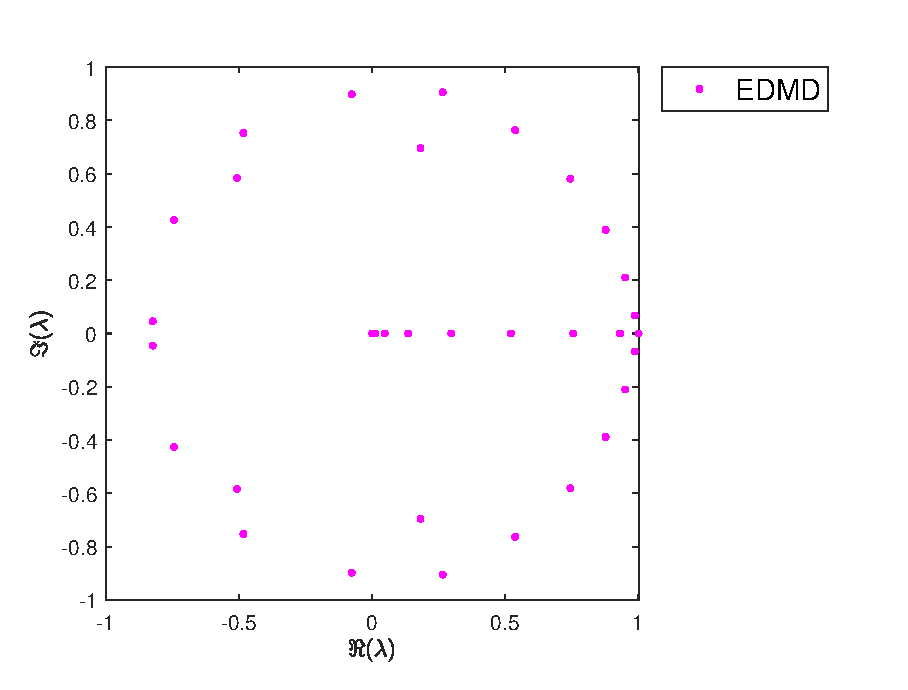
\includegraphics[width=0.98\linewidth]{../code/figures/gauss_map/presentation_edmd.eps}
  \end{subfigure}\hfill
  \uncover<2>{
  \begin{subfigure}{.49\linewidth}
    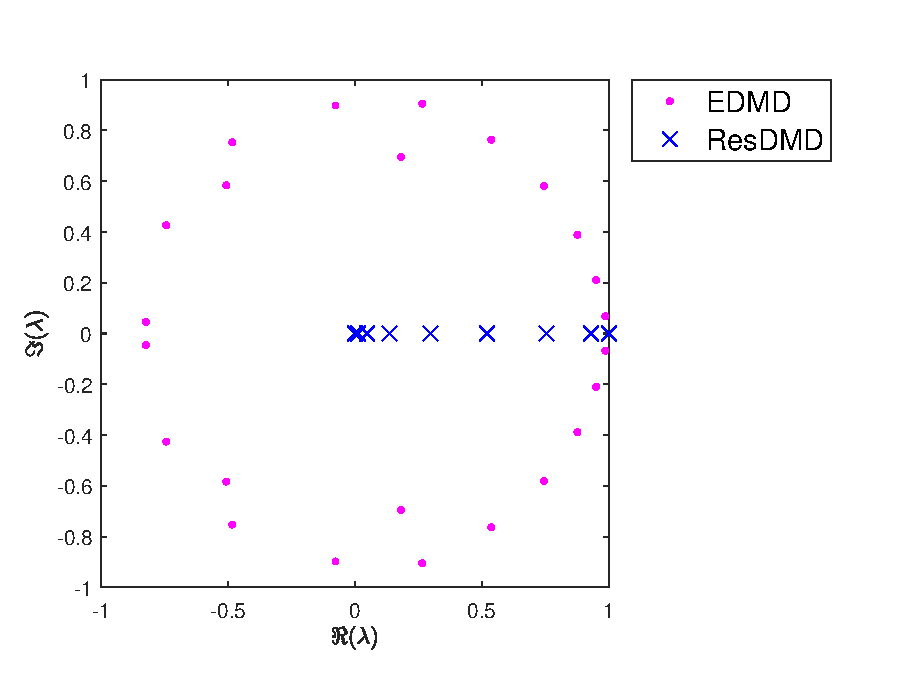
\includegraphics[width=\linewidth]{../code/figures/gauss_map/presentation_resdmd.eps}
  \end{subfigure}}\\
\end{figure}
\end{frame}

\note[itemize]{\item ResDMD retains only the eigenvalues represented by blue crosses.}

\begin{frame}{ResDMD to approximate the pseudospectrum}
\only<1>{
\begin{definition}[Pseudospectrum]
\begin{itemize}
    \item Square matrices: $\displaystyle{\sigma_{\varepsilon}(\vb{A}) = \left\{ \lambda\in\C \text{ : } \norm{(\vb{A} - \lambda \vb{I})^{-1}}_2 \geq \frac{1}{\varepsilon}\right\}}$
    %\item Rectangular pencils: $\displaystyle{\sigma_{\varepsilon}(\vb{A}, \vb{B}) = \left\{ \lambda\in\C \text{ : } \sigma_{\mathrm{min}}(\vb{A} - \lambda \vb{B}) \leq \varepsilon \right\}}$
    \item Koopman Operator: $\displaystyle{\sigma_{\varepsilon}(\mathcal{K}) = \mathrm{cl}\left( \left\{ \lambda\in\C \text{ : } \norm{(\mathcal{K} - \lambda \cdot \mathrm{id})^{-1}} > \frac{1}{\varepsilon}\right\} \right)}$
\end{itemize}
\end{definition}

\structure{\textbf{ResDMD for pseudospectrum approximation:}} For each $\lambda$ on a grid, compute the function $\phi\in\Span(\mathcal{D})$ that minimizes (an approximation of) $\mathrm{res}(\lambda, \phi)$ and keep $\lambda$ if $\mathrm{res}(\lambda, \phi)<\varepsilon$.
\begin{prop}[\cite{colbrook_rigorous_2021}, Theorem 4.1]
Assuming that the quadrature rule converges, then for each $\lambda$ in output to ResDMD it holds: 
\begin{equation*}
    \limsup_{M\to+\infty} \max_{\lambda\in\Lambda}\norm{(\mathcal{K} - \lambda\cdot \mathrm{id})^{-1}}^{-1} \leq \epsilon.
\end{equation*}
\end{prop}}
\end{frame}
\note[itemize]{
\item Pseudospectra are a tool that allow us to detect this so called spectral pollution and to define trust regions for the approximation of the eigenvalues.
\item In spite of the fact that the eigenvalues returned by Algorithm 4 lie in the $\epsilon$-pseudospectrum (in the large data limit), the eigenvalues of K might not approximate the whole spectrum of K and therefore it might not be possible to approximate the whole $\epsilon$-pseudospectrum of K using Algorithm 4. A simple modification of Algorithm 4 allows us to draw an approximation of the $\epsilon$-pseudospectrum of K starting from a grid of points in the complex plane.
}

\begin{frame}[fragile]{An example of pseudospectrum approximation}
\only<1>{
\begin{figure}[h]
    \begin{center}
        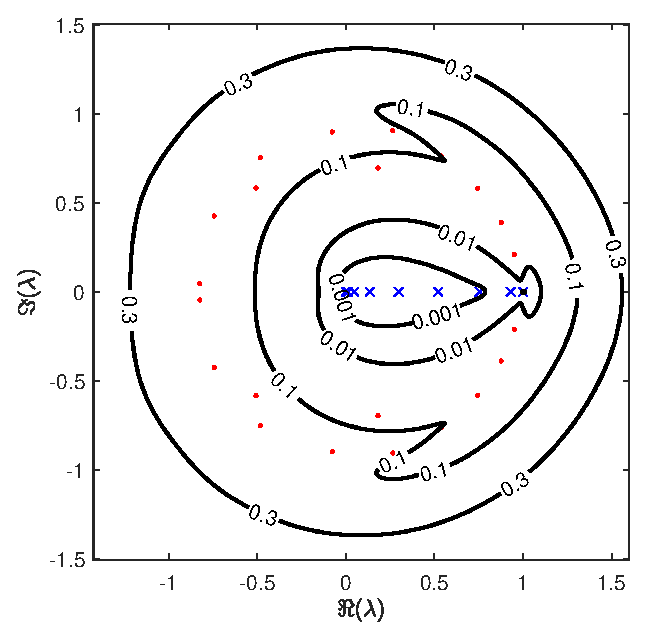
\includegraphics[width=0.55\linewidth]{../code/figures/gauss_map/pseudospectra_contour.eps}
    \end{center}
    \caption{Gauss iterated map problem. Contour lines of the $\varepsilon$-pseudospectrum for $\varepsilon = 0.3,\,0.1,\,0.01,\,0.001$ computed using ResDMD with dictionary of $K=40$ observables.}
\end{figure}
}
\end{frame}


\begin{frame}{Kernelized EDMD (K-EDMD)}
\alert{\textbf{Limitation of EDMD (and ResDMD):}} Need to find a suitable dictionary for each problem.

\medskip
\structure{\textbf{Possible solution:}} Start from a general purpose kernel, such as RBF, and use a two-steps extraction procedure.
\begin{figure}[h]
    \begin{center}
        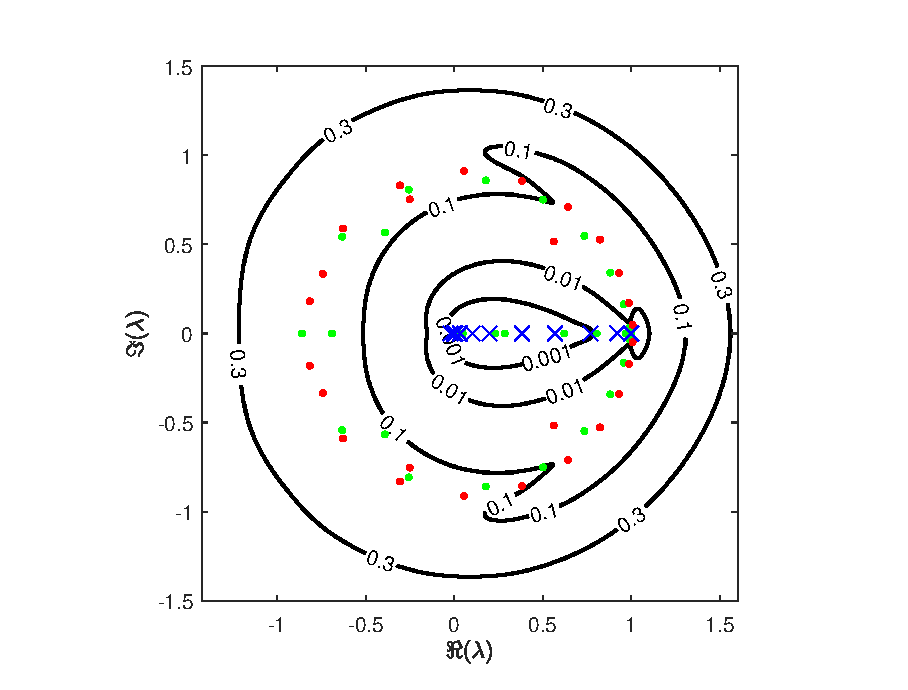
\includegraphics[width=0.50\linewidth]{../code/figures/gauss_map/kernelized/presentation.eps}
    \end{center}
    \caption{Output of Kernelized ResDMD starting from the RBF kernel and Montecarlo quadrature nodes. Pseudospectral countour lines obtained with standard ResDMD are plotted as a reference.}
\end{figure}
\end{frame}

\note[itemize]{
\item KEDMD has been originally applied to high-dimensional problems where, to approximate the Koopman spectrum, one needs a dictionary size larger than the number of snapshots. This leads to a modification of ResDMD that requires a two step procedure. 
\item However, one of the limitations of EDMD is the need to define a suitable dictionary to each problem.
\item We applied the previously mentioned two-steps procedure to the Gauss iterated map problem in order to obtain approximations of the Koopman eigenvalues without the need of a hand-crafted dictionary. We can see that the results are very similar to the ones obtained using the previous approach.
}

\begin{frame}{Summary}
\structure{\textbf{Koopman Operator}}:
\begin{itemize}
    \item linear operator, also for nonlinear dynamics
    \item \alert{but} infinite dimensional
\end{itemize}
\structure{\textbf{DMD}}:
\begin{itemize}
    \item equivalent to Arnoldi for linear dynamics
    \item \alert{but} less numerically stable: use the SVD-based version
    \item not suited for nonlinear dynamics
\end{itemize}
\structure{\textbf{EDMD/ResDMD}}:
\begin{itemize}
    \item tailored for the Koopman operator
    \item spectral pollution problem: use \structure{ResDMD}
    \item \structure{ResDMD} can be used for approximating the Koopman pseudospectrum 
\end{itemize}
\end{frame}


\begin{frame}{Main references}
\nocite{*}
\printbibliography
\end{frame}
\end{document}